\chapter{Signalerzeugung und Kanalsimulation}
\label{chap:Signalerzeugung}

In diesem Kapitel sollen die in der Simulation verwendeten Signal-Parameter und -Erzeugung erläutert werden. Anschließend wird die Implementierung des Kanals kurz umrissen.

\section{Simulationsparameter}
\label{chap4.1:Simulationsparameter}
In Abschnitt \ref{chap2.4:Signalcharakteristik} wurde bereits erklärt, wie Mehrtonsignale erzeugt werden können. In diesem Abschnitt werden deren Parameter für die Simulation festgelegt. 

\begin{itemize}
\item Signaldauer $T \approx \unit[0.5]{ms} $ 
\item Trägerfrequenz $f_c = \unit[868]{MHz}$
\item Bandbreite B $\equiv$ Chiprate $f_{chip} = \unit[2]{MHz}$
\item Abtastfrequenz $f_{sampling} = \unit[4]{MHz}$
\end{itemize}

Die Signaldauer hängt bei der Simulation von der Bandbreite \gls{symb:B} und der Anzahl der Symbole im Signal ab. 
Es wurde $\unit[2]{MHz}$ als Bandbreite gewählt, da dies die Standard-Bandbreite im $\unit[868]{MHz}$-Band ist.   
Ein  Chip entspricht einem Symbol in der Sequenz. Wenn die Chiprate $f_{chip} = \unit[2]{MHz}$ sein soll, dann beträgt die Symboldauer eines Chips $\unit[0.5]{\mu s}$. Die Wellenlänge der Trägerfrequenz ist $\lambda = \frac{c_0}{f} = \unit[35]{cm}$. Damit passen $428,6$ Schwingungen in einen Chip. Um eine geeignete Abtastfrequenz zu finden, muss zunächst das Nyquist-Shannon-Abtasttheorem erfüllt sein.  
 
\begin{equation}
	 \label{eq:Abtasttheorem}
	 f_{sampling} \geq 2\cdot \gls{symb:B}
\end{equation}

Da die Bandbreite $\unit[2]{MHz}$ beträgt, muss \gls{symb:fc} mindestens $\unit[4]{MHz}$ sein. Die Auswirkungen der Bandvergrößerung werden im folgenden Kapitel genauer erläutert.

\section{Signalerzeugung}
\label{chap4.2:Signalerzeugung}
Für die Auswertung wurden fünf Subträgerverteilungen im gegebenen Band ausgewählt. Aus den Hadamard-Sequenzen wurde ein 4-Ton, 8-Ton und 16-Ton verwendet. Die Spektren dieser vier Sequenzen sehen wie folgt aus:

\begin{figure}[htbp]
	\centering
	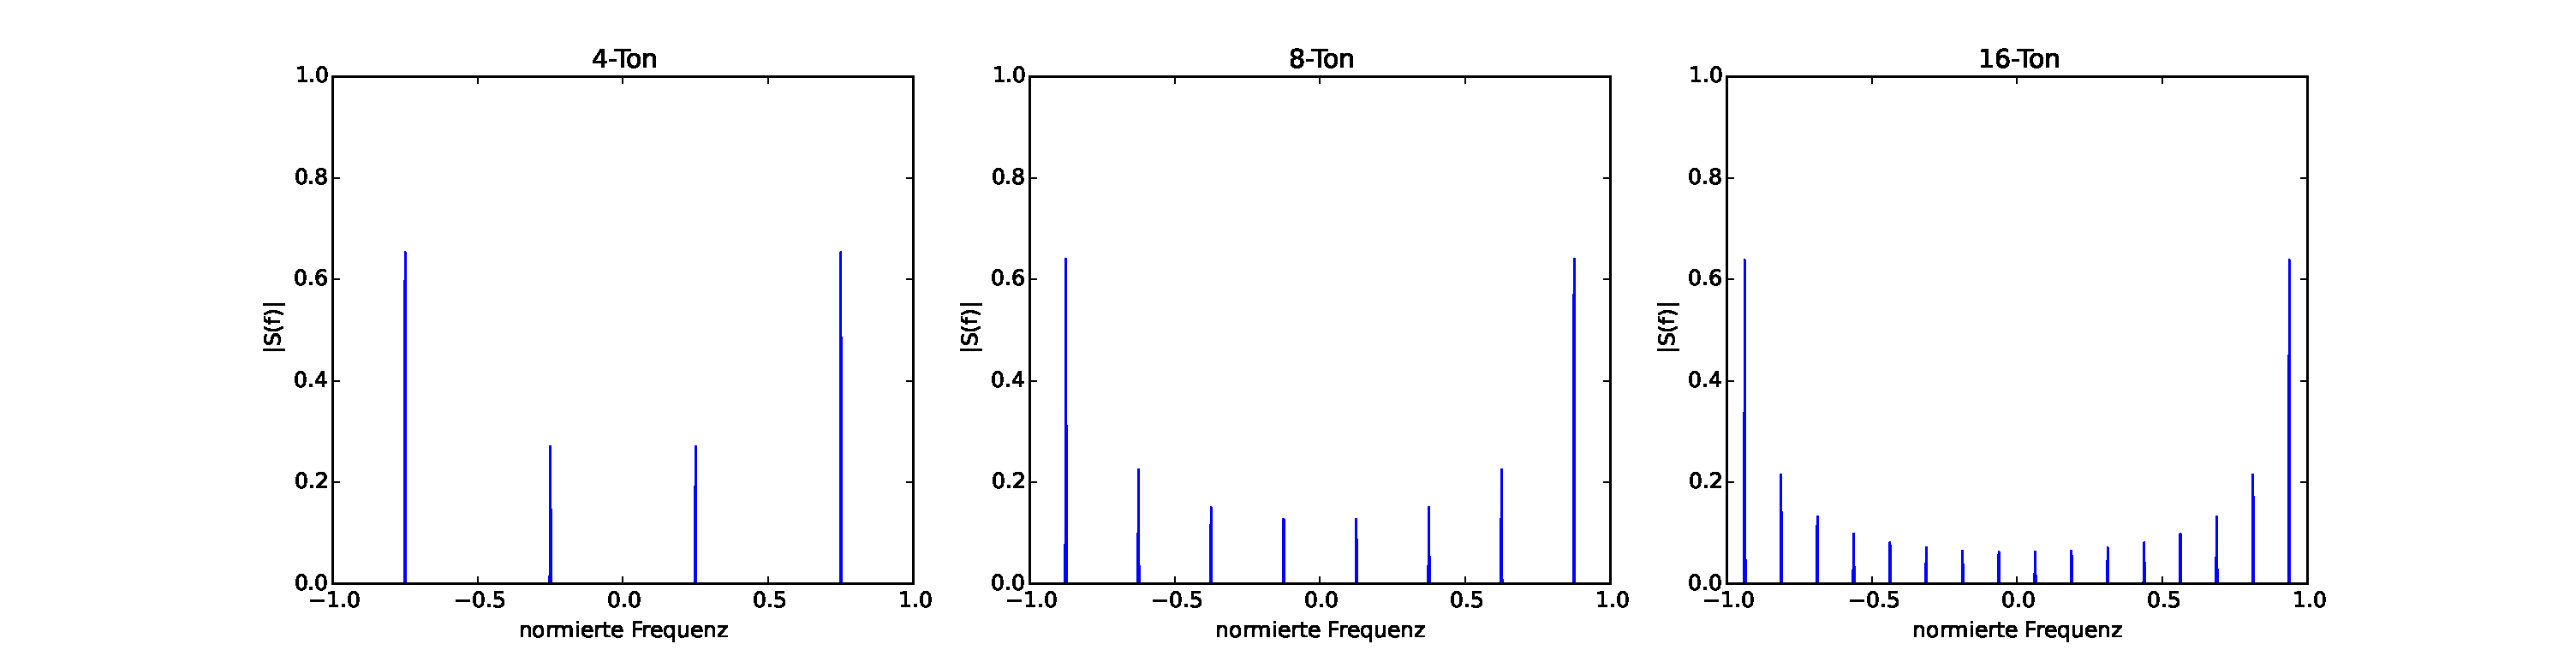
\includegraphics[width = \textwidth]{images/HadamardBeispiel}
	\caption{Normiertes Betragsspektrum der verwendeten Hadamard-Sequenzen}
	\label{fig:HadamardBeispiel}
\end{figure}
Es wurde darauf geachtet, dass die Subträger an den Bandkanten stärker gewichtet sind um die \gls{CRLB} der der Signale so klein wie möglich zu halten. Betrachtet man den 16-Ton, sieht er dem 8-Ton sehr ähnlich. Die äußeren beiden Subträger haben jedoch die gleiche Gewichtung wie der 8-Ton. Je mehr man in die Bandmitte geht, desto weniger stark sind die Subträger gewichtet.

Aus den $m$-Sequenzen wurde eine Sequenz der Länge 7 und eine der Länge 1023 gewählt. Dementsprechend viele Subträger haben sie.  
\begin{figure}[htbp]
	\centering
	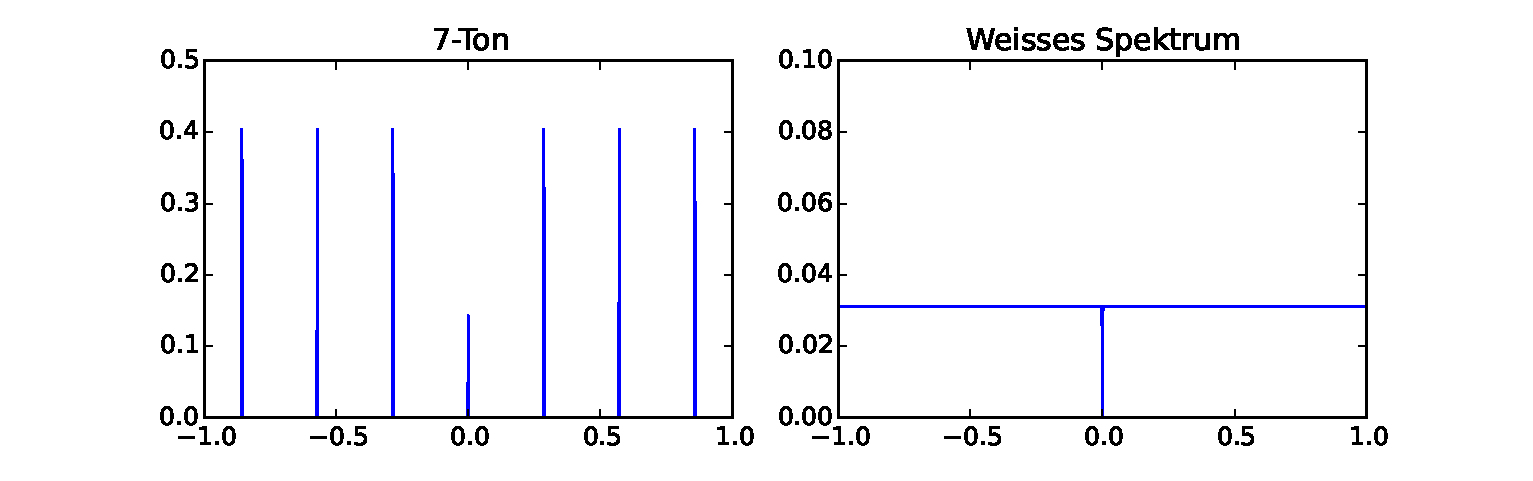
\includegraphics[width = \textwidth]{images/mSeqBeispiel}
	\caption{Normiertes Betragsspektrum der verwendeten $m$-Sequenzen}
	\label{fig:mSeqBeispiel}
\end{figure}
Die x-Achse entspricht wieder der normierten Frequenz und die y-Achse einem normierten Betragsspektrum. Auffällig ist, dass Beträge der Subträger bei $m$-Sequenzen wesentlich niedriger sind. Da nach dem Theorem von Parseval, die Summe über dem quadratischen Betragsspektrum, die Energie des Signals ergibt, zeigen die Spektren der $m$-Sequenzen, dass die Energie stärker verteilt ist.

Damit aus diesen Sequenzen Signale entstehen, muss eine Impulsformung stattfinden.
Als Modulationsimpuls wurde ein Rechteck verwendet. Da ein ideales Rechteck ein unendlich langes Spektrum besitzt, kann dieses als Modulationsimpuls nicht realisiert werden. Anstatt dessen, wird eine Näherung vorgenommen. Ein Rechteck, welches beispielsweise mit zwei diskreten Werten abgetastet wird, ist bandbegrenzt.  
Die Fouriertransformation eines Rechtecks ist eine Sinc-Funktion.
Deshalb folgt aus der Modulation mit einem Rechteckimpuls, eine Multiplikation des Spektrums mit einer Sinc-Funktion. Je höher dieses Rechteck abgetastet wird, desto breiter ist die Sinc-Funktion im Frequenzbereich. Da unsere Chiprate $f_{chip} = \unit[2]{MHz}$ beträgt, muss die Rate, mit der das Rechteck abgetastet wird, $\unit[4]{MHz}$ betragen, was auch der Breite der Sinc-Funktion entspricht. Aus einer diskreten Folge,  wird ein periodisches Spektrum erzeugt. Diese Periodizität ist in den Abbildungen \ref{fig:HadamardBeispiel} und \ref{fig:mSeqBeispiel} nicht zu erkennen, da die Abbildungen auf eine Periode bandbegrenzt sind. Das Spektrum des Rechtecks ist jedoch doppelt so breit wie in den vorherigen Abbildungen, deshalb werden die periodisch fortgesetzten Spektren mit dem Außenbereich der Hauptkeule der Sinc-Funktion gewichtet. Dieses Phänomen ist in Abbildung \ref{Modspek} verdeutlicht.

\begin{figure}[htbp] 
	\centering
	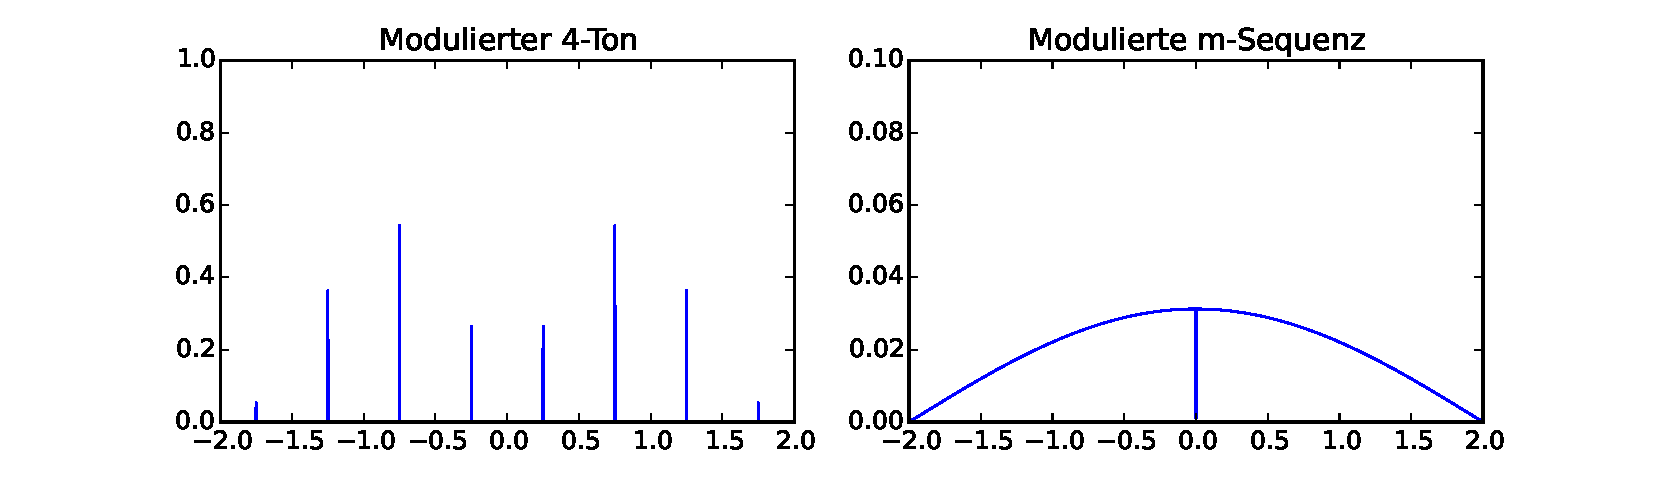
\includegraphics[width = \textwidth]{images/Modspek}
	\caption{Spektrum eines 4-Ton und einer $m$-Sequenz mit weißem Spektrum, moduliert mit einem Rechteck im Zeitbereich}
	\label{Modspek}
\end{figure}

Am Spektrum der modulierten m-Sequenz ist die Hauptkeule der Sinc-Funktion äußerst gut zu erkennen. Dieses Spektrum ist nun nicht mehr weiß. Am Spektrum des 4-Tons kann auch, außerhalb des $\unit[2]{MHz}$ Bandes, die gewichteten periodischen Wiederholungen beobachtet werden. Es befinden sich nun mehr Träger im Band, als gewollt. Deshalb muss nochmals bandbegrenzt werden. Auch nach der Bandbegrenzung ist ein kleiner Einfluss der Sinc-Funktion geblieben. Es muss beachtet werden, dass dieser Einfluss die effektive Bandbreite \gls{symb:brms} der Signale nach der Impulsformung verschlechtert hat, da die Subträger an den Bandkanten gestaucht werden. 

\section{Kanalsimulation}
\label{chap4.3:Kanalsimulation}

In Abschnitt \ref{chap2.2:Kanalmodell} wurden bereits die verwendeten Kanalmodelle vorgestellt. Jedes der verwendeten Modelle besteht aus einem Verzögerungsglied um die Laufzeit darzustellen. Die softwareseitige Realisierung einer Verzögerung der diskreten Folge ist allerdings von den Abtastwerten, \emph{Samples}, abhängig. Um die Folge zu verzögern, muss sie um n-Abtastwerte verschoben werden. Die kleinstmögliche Verzögerung die dabei bewerkstelligt werden kann, ist die um ein \emph{Sample}. Haben wir Beispielsweise eine Abtastrate von $ f_{sampling} = \unit[2]{MHz}$, dann sind zwei benachbarte Abtastwerte $\frac{1}{f_{sampling}} = \unit[0,5]{\mu s}$ bzw. $\unit[150]{m}$  voneinander entfernt. Dies ist allerdings zum Testen der Algorithmen nicht zielführend, da Mehrwegestörungen schon bei geringeren Distanzen auftreten. Deshalb muss eine Möglichkeit gefunden werden, einen Umwegpfad zu simulieren, der kürzer als $\unit[150]{m}$ ist. Um eine Verzögerung im Subsamplebereich zu realisieren, bietet es sich an, ein \emph{Fractional-Delay-Filter} zu verwenden. 

\subsection{Fractional-Delay-Filter (FD-Filter)}
\label{chap4.3.1:FD-Filter}
Um einen solchen Filter zu entwerfen, muss die Übertragungsfunktion einer Verzögerung in den Zeitbereich zurück transformiert werden. In Formel \ref{eq:Verschiebungssatz} sehen wir, dass die Übertragungsfunktion $H(e^{j\omega}) = e^{-j\omega D}$ ist, wobei $D$ den Verzögerungswert in Samples darstellt\cite{fd-filter}. $D$ kann in einen ganz- und gebrochenzahligen Anteil zerlegt werden. Die inverse Fouriertransformation dieser Übertragungsfunktion ergibt die, in \eqref{eq:Impulsresponse} zu sehende diskrete Impulsantwort. 

\begin{equation}
	\label{eq:Impulsresponse}
	h[n] = \frac{\sin(\pi(n-D))}{\pi(n-D)} = sinc[n-D]
\end{equation}

Die Impulsantwort muss mit dem Sendesignal gefaltet werden. Wenn $D$ ganzzahlig ist, geht die Funktion $sinc(n-D)$ in einen Dirac-Impuls bei $D$ über. Die Faltung ist folglich wie gewünscht eine Verschiebung um $D$. Wenn $D$ nicht ganzzahlig ist, wird die Sinc-Funktion um den ganzzahligen Anteil verschoben und versetzt abgetastet, was zu einer unendlichen Folge skalierter Dirac-Impulse führt. Das beantwortet die Frage, wo der verzögerte Signalwert liegt, da er sich nicht zwischen zwei Abtastwerten befinden kann. Im Idealfall sollte der Wert über das ganze Signal mit entsprechender Gewichtung verteilt werden. Gewichtet wird durch die Sinc-Funktion. In Abbildung \ref{fig:Sinc} wird dies beispielhaft für $D = 2$ und $D = 2.3$ dargestellt.

\begin{figure}[htbp]
	\centering
	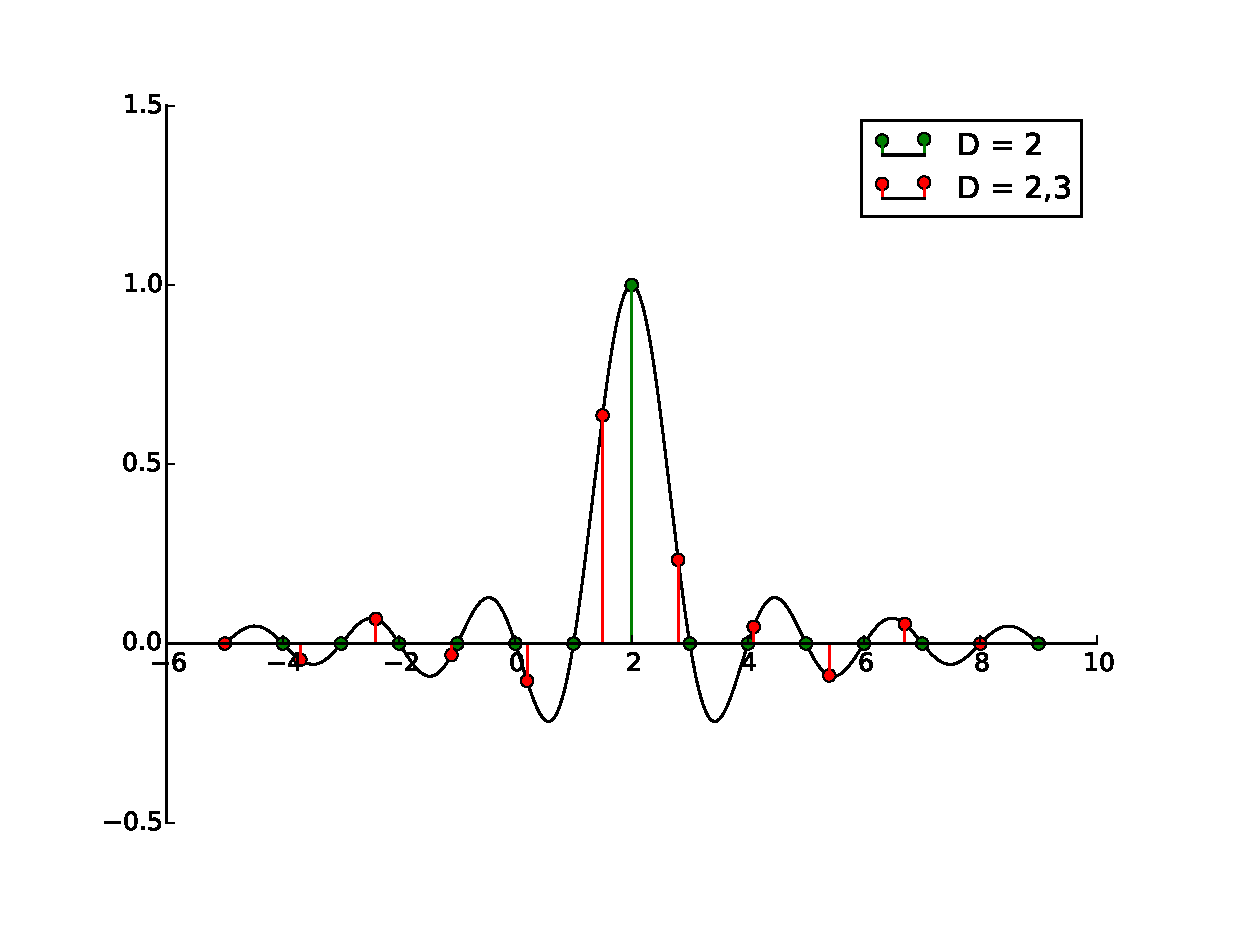
\includegraphics[scale=0.5]{images/Sinc}
	\caption{Impulsantwort eines Fractional Delay Filters}
	\label{fig:Sinc}
\end{figure}

Die ideale Impulsantwort ist, aufgrund ihrer Unendlichkeit, nicht realisierbar. Sie muss an irgendeinem Punkt abgeschnitten werden. Dies führt zu einem Ripple-Effekt im Frequenzbereich, welcher auch Gibb'sches Phänomen genannt wird. Dieser Effekt kann durch Wahl einer geeigneten Fensterfunktion minimiert werden.

\subsection{Implementierung}
Bei der konkreten Implementation wurde die Phase, mithilfe der Verzögerung, direkt im Frequenzbereich moduliert, und anschließend mit einer Rücktransformation die entsprechende Sinc-Funktion erzeugt. Da der Frequenzbereich der modulierten Exponentialfunktion auf das verwendetet Band begrenzt wurde, ist die Sinc-Funktion entsprechend gefenstert. In \cite{fd-filter} wurde dieses Fenster hergeleitet und sieht wie folgt aus:

\begin{equation}
	\label{eq:fd-window}
	w[n] = \frac{cos\left(\frac{\pi (n-D)}{N}\right)}{sinc\left(\frac{n-D}{N}\right)}  \;\;\; mit \;\;\; 0 \leq n \leq (N-1)
\end{equation}

Der Mehrwegekanal besteht aus Summation mehrerer gewichteter \gls{FD}, die mit einer zusätzlichen Exponentialfunktion multipliziert wurden, um die Reflektorphase zu berücksichtigen.  




 
